\begin{figure}[t]
  \centering
  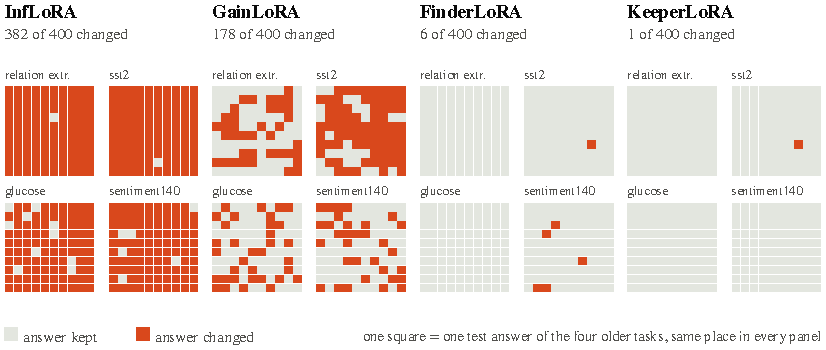
\includegraphics[width=\linewidth]{figures/answer_grid}
  \caption{Every square is one test answer. Five tasks without definitions, \AudFullEpochs{}
  epochs per task, seed 42: the \AudFullCompared{} test answers of the four older tasks, right
  after their task was learned against after the last task; a square has the same place in every
  panel. InfLoRA changes \AudFullInfloraChanged{} of the \AudFullCompared{} answers, GainLoRA
  \AudFullGainloraChanged{}, \recog{} \AudFullOursRidgeChanged{} and \handicap{}
  \AudFullOursHandicapChanged{}.}
  \label{fig:answergrid}
\end{figure}
